\documentclass[12pt]{article}
\usepackage{tikz}
\usetikzlibrary{calc}
\title{An Implementation of Halfedge Data Structure in Catmull-Clark 
Subdivision for 2-Manifold Single-sided Surface}
\author{Yu Wang}
\date{August 2015}

\begin{document}
\maketitle
\newpage

%\begin{abstract} A place for abstract later
% Contents of abstract
%\end{abstract}

\section{Introduction}
Catmull-Clark Subdivision is a 
\section{Halfedge Data Structure} \label{sec:halfedge}

An object in 3D Euclid space can be represented by multiple meshes of polygons. 
A mesh comprises three types of geometry element: vertex, edge, and face. 
The adjacency structure stores the topological information (adjacency and 
connectivity) of the mesh. The author chose halfedge data structure as the 
adjacency structure in this project to realize Catmull-Clark subdivision.

\subsection{Vertex, Halfedge, and Face}

The definitions and assumptions of vertex, halfedge and face are shown 
in Table \ref{table:vhfdef}. A quadrilateral face made with four halfedges 
is shown in Figure \ref{figure:singleFace}. 

%Table1
\begin{table}[ht]
\centering
\begin{tabular}{| l | p{0.4\textwidth} | p{0.4\textwidth}|}

\hline
		&	Definition	& Assumption	\\
\hline
Vertex	&	A 3-dimensional point.		&	No overlapping vertices 
exits in a mesh. But overlapping vertices can exist in different meshes.\\
\hline
Halfedge	&	An edge that starts from one vertex and end at another vertex. & 
A halfedge connects exactly two non-overlapping vertices and it has a direction. 
Less than two halfedges start from the same vertex and end at the same vertex in a 
single mesh.\\
\hline
Face		&	A polygon that contains a loop of vertices and halfedges.	& A face has at 
least three non-overlapping vertices so it makes a polygon. The face has to be constructed 
with a complete loop of halfedges with on openings.\\
\hline
\end{tabular}
\caption{Definitions and assumptions of vertex, halfedge, and face} 
\label{table:vhfdef}
\end{table}

%Figure1
\begin{figure}[ht]
  \centering
  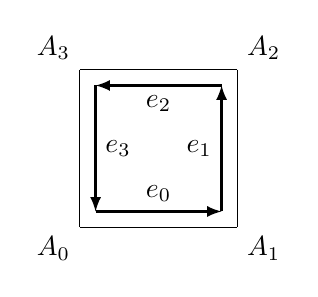
\begin{tikzpicture}
    \coordinate (A0) at (0,0);
    \coordinate (A1) at (2,0);
    \coordinate (A2) at (2,2);
    \coordinate (A3) at (0,2);
    \coordinate (B0) at (0.2,0.2);
    \coordinate (B1) at (1.8,0.2);
    \coordinate (B2) at (1.8,1.8);
    \coordinate (B3) at (0.2,1.8);
      \draw(A0)
        -- (A1) node [below right] {$A_1$};
      \draw (A1)
        -- (A2) node [above right] {$A_2$};
      \draw (A2)
        -- (A3) node [above left] {$A_3$};
      \draw (A3)
        -- (A0) node [below left] {$A_0$};
      \draw  [thick,-latex] (B0)
        -- (B1);
      \draw [thick,-latex,] (B1)
        -- (B2);
      \draw [thick,-latex,] (B2)
        -- (B3);
      \draw [thick,-latex,] (B3)
        -- (B0);
      \node [right] at (0.2, 1) {$e_3$};
      \node [above] at (1, 0.2) {$e_0$};
      \node [left] at (1.8, 1) {$e_1$};
      \node [below] at (1, 1.8) {$e_2$};
  \end{tikzpicture}
  \caption{A quadrilateral face made with four halfedges}
  \label{figure:singleFace}
\end{figure}

The vertex, halfedge, and face store their own information and pointers to the adjacent elements. The information that these elements store can be classifed into self-information and adjacency information, which is shown in Table \ref{table:vhfInfo}
%Table2
\begin{table}[ht]
\centering
\begin{tabular}{| l | p{0.4\textwidth} | p{0.4\textwidth}|}

\hline
Element & Self-Information & Adjacency Information  \\
\hline
Vertex  & vertex position & one outgoing halfedge   \\
& vertex normal & \\
& vertex ID & \\
\hline
Halfedge & & start vertex and end vertex\\
& & the face it belongs to\\
& & predecessor and successor halfedge in the face\\
& & sibling links to adjacent face\\
& & boundary links to adjacent face \\
\hline
Face    &  face normal & vertices of the face.\\ %(Redundant, should be delete later.)\\
& & one side halfedge\\
\hline
\end{tabular}
\caption{Definitions and assumptions of vertex, halfedge, and face} 
\label{table:vhfInfo}
\end{table}


\subsection{Face Connections}

There are two types of face connections, the normal connection and the mobius connection, as shown in Figure \ref{figure:faceConnections}

%Figure2
\begin{figure}[ht]
  \centering
  %Normal Junction
  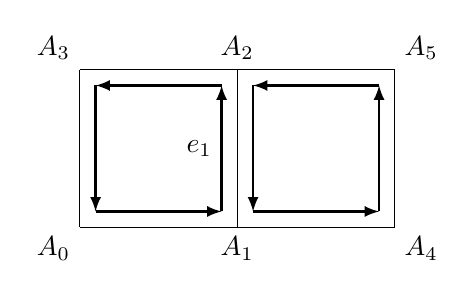
\begin{tikzpicture}
    \coordinate (A0) at (0,0);
    \coordinate (A1) at (2,0);
    \coordinate (A2) at (2,2);
    \coordinate (A3) at (0,2);
    \coordinate (A4) at (4,0);
    \coordinate (A5) at (4,2);
    \coordinate (B0) at (0.2,0.2);
    \coordinate (B1) at (1.8,0.2);
    \coordinate (B2) at (1.8,1.8);
    \coordinate (B3) at (0.2,1.8);
    \coordinate (B4) at (2.2,0.2);
    \coordinate (B5) at (3.8,0.2);
    \coordinate (B6) at (3.8,1.8);
    \coordinate (B7) at (2.2,1.8);
      \draw(A0) -- (A1) node [below] {$A_1$};
      \draw (A1) -- (A2) node [above] {$A_2$};
      \draw (A2) -- (A3) node [above left] {$A_3$};
      \draw (A3) -- (A0) node [below left] {$A_0$};
      \draw (A1) -- (A4) node [below right] {$A_4$};
      \draw (A4) -- (A5) node [above right] {$A_5$};
      \draw (A5) -- (A2);
      \draw  [thick,-latex] (B0)
        -- (B1);
      \draw [thick,-latex,] (B1)
        -- (B2);
      \draw [thick,-latex,] (B2)
        -- (B3);
      \draw [thick,-latex,] (B3)
        -- (B0);
      \draw  [thick,-latex] (B4)
        -- (B5);
      \draw [thick,-latex,] (B5)
        -- (B6);
      \draw [thick,-latex,] (B6)
        -- (B7);
      \draw [thick,-latex,] (B7)
        -- (B4);
      \node [left] at (1.8, 1) {$e_1$};
  \end{tikzpicture}
  
  %Mobius Junction
  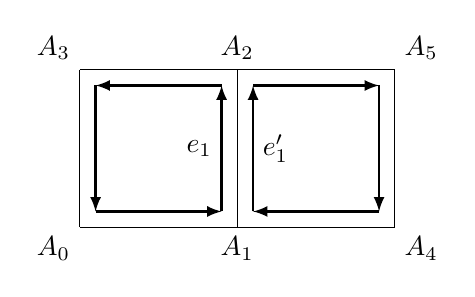
\begin{tikzpicture}
    \coordinate (A0) at (0,0);
    \coordinate (A1) at (2,0);
    \coordinate (A2) at (2,2);
    \coordinate (A3) at (0,2);
    \coordinate (A4) at (4,0);
    \coordinate (A5) at (4,2);
    \coordinate (B0) at (0.2,0.2);
    \coordinate (B1) at (1.8,0.2);
    \coordinate (B2) at (1.8,1.8);
    \coordinate (B3) at (0.2,1.8);
    \coordinate (B4) at (2.2,0.2);
    \coordinate (B5) at (3.8,0.2);
    \coordinate (B6) at (3.8,1.8);
    \coordinate (B7) at (2.2,1.8);
      \draw(A0) -- (A1) node [below] {$A_1$};
      \draw (A1) -- (A2) node [above] {$A_2$};
      \draw (A2) -- (A3) node [above left] {$A_3$};
      \draw (A3) -- (A0) node [below left] {$A_0$};
      \draw (A1) -- (A4) node [below right] {$A_4$};
      \draw (A4) -- (A5) node [above right] {$A_5$};
      \draw (A5) -- (A2);
      \draw  [thick,-latex] (B0)
        -- (B1);
      \draw [thick,-latex,] (B1)
        -- (B2);
      \draw [thick,-latex,] (B2)
        -- (B3);
      \draw [thick,-latex,] (B3)
        -- (B0);
      \draw  [thick,-latex] (B5)
        -- (B4);
      \draw [thick,-latex,] (B4)
        -- (B7);
      \draw [thick,-latex,] (B7)
        -- (B6);
      \draw [thick,-latex,] (B6)
        -- (B5);
      \node [left] at (1.8, 1) {$e_1$};
      \node [right] at (2.2, 1) {$e_1'$};
  \end{tikzpicture}
  \caption{Normal junction (left) and mobius junction (right) between two faces}
  \label{figure:faceConnections}
\end{figure}

\subsection{Build a Mesh}

\subsubsection{Build from Elements}
\subsubsection{Instantiation and Rotation}
\subsubsection{Build by Merging Meshes}

\section{Catumll-Clark Subdivision} \label{sec:ccsd}

\subsection{General Approach of Catmull-Clark Subdivision}

\subsubsection{Compute Vertex Positions of New Mesh}

\subsubsection{Make Connections of New Mesh}

\subsection{Sharp Crease and Boundary Feature}

\subsection{Mobius Connection}

\section{Offset Surface} \label{sec:offset}

\subsection{Compute Vertex Normals}

\subsection{Positive and Negative Offsets}

\subsection{Mobius Connection Issue}


\section{Test Cases and Discussions}



\section{Contribution to Knowledge}




\section{Future Researches}


\end{document}